\definecolor{Gray}{gray}{0.9}

\chapter{Analisi del dominio}
Questo capitolo verte su tutta l'analisi impiegata sulla conoscenza del dominio dell'applicativo, sull'identificazione dei requisiti, dei casi d'uso nonché sull'analisi dei principi della filosofia Domain Driven Design. \newline \newline Questa fase è stata di grande importanza poiché ci ha permesso, da una parte di avere un ottima conoscenza del dominio applicativo e dall'altra di discutere sui principali aspetti di sviluppo agevolando notevolmente la successiva fase di implementazione.

\section{Il dominio}
In questa sezione verrà descritto il dominio dell'applicativo: verrà presentato l'obiettivo da raggiungere, lo stato dell'arte e l'\textit{ubiquitous language} individuato.
 
\subsection{Obiettivo}

L'obiettivo del progetto è la creazione di un sistema che consenta a tutto il team della sala operatoria (medici, infermieri e anestesisti) di accedere in maniera agevole a tutte le informazioni del paziente durante un intervento chirurgico. In particolare quello che si richiede è di poter digitalizzare attraverso un ologramma il monitor a parametri vitali del paziente. In questo modo, durante un intervento, ogni membro del team può visualizzare il proprio ologramma controllando i relativi valori dei parametri del monitor indipendentemente dalla locazione del dispositivo fisico. \newline \newline Questo approccio porta a semplificare tutte una serie di operazioni che possono essere svolte sul paziente durante l'operazione. Si pensi se durante un intervento è necessario eseguire una TAC d'urgenza: significherebbe trasportare il paziente, tutti i sensori a cui è collegato e il relativo monitor in una stanza adiacente a quella chirurgica con il rischio di perdere del tempo prezioso per problemi che possono incorrere durante il trasferimento. Se si adottasse la soluzione proposta, sarebbe necessario spostare solamente il paziente e non i dispositivi fisici poiché ogni membro del team continua a visualizzare l'ologramma minimizzando il tempo impiegato nel trasferimento del paziente.
Un altro vantaggio è dato dalla connessione in remoto allo stato del monitor del paziente da parte di altri medici che possono essere coinvolti nell'operazione.

\subsection{Stato dell'arte}
Molte grandi città del mondo stanno già impiegando questa tecnologia in ambito sanitario. Ad esempio nell'ospedale di Singapore, i chirurgi utilizzano questo approccio per visualizzare ologrammi di referti dei pazienti, come una risonanza magnetica, durante un intervento chirurgico (maggiori informazioni a questo \href{https://govinsider.asia/citizen-centric/how-a-singapore-hospital-uses-holograms-to-assist-surgery-nuhs-ngiam-kee-yuan/}{link}). Si tratta di un caso simile al nostro ma non del tutto identico. 
La differenza è dovuta al contenuto dell'ologramma cioè quale oggetto tridimensionale si vuole riprodurre nello spazio: nel nostro caso si tratta di un monitor a parametri viali.

\begin{wrapfigure}{l}{0.4\textwidth}
    \centering
    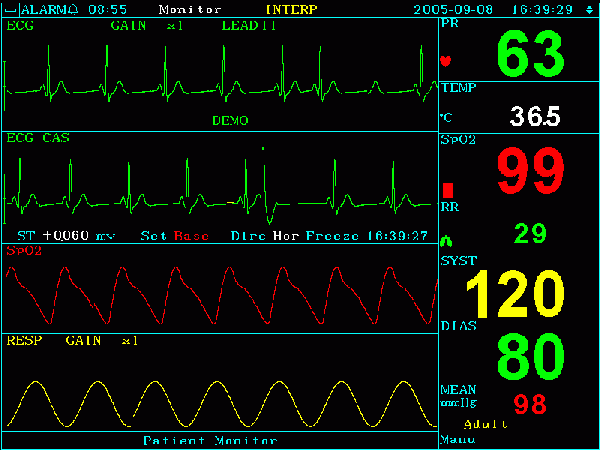
\includegraphics[width=0.4\textwidth]{monitor.png}
\end{wrapfigure}

Durante l'intervento, al paziente vengono collegati diversi sensori per monitorare i parametri vitali.
I valori dei parametri vengono mostrati nel monitor ognuno con uno specifico colore. In particolare per ogni parametro viene mostrato il valore puntuale, l'unità di misura e per alcuni di loro anche un grafico. 
A sinistra è presente un esempio di monitor a parametri vitali ed è quello a cui noi ci siamo basati per la parte di simulazione. I parametri vitali monitorati sono: temperatura, pressione sanguigna, frequenza respiratoria, frequenza cardiaca e saturazione. Per ognuno di questi si è deciso anche di aggiungere un allarme che si attiva qualora il relativo valore supera una certa soglia sia inferiormente che superiormente.

\subsection{Ubiquitous Language}
L'\textit{ubiquitous language} è un dizionario comune di termini usati nella definizione del dominio al fine di eliminare incertezze, imprecisioni e fraintendimenti che possono derivare da ogni membro del team di progetto, esperti del dominio e altri partecipanti. Tale linguaggio è sempre in continuo aggiornamento anche durante tutta la fase di sviluppo e non definito solamente all'inizio. \newline \newline Di seguito è illustrato l'\textit{ubiquitous language} per il nostro applicativo in base al contesto in cui viene utilizzato. Sono presenti tre tabelle: nella tabella \ref{tab:phisical-asset-ubiquitous-language-table} è riportato  l'\textit{ubiquitous language} di termini legati all'asset fisico, la tabella \ref{tab:general-ubiquitous-language-table} descrive termini di carattere generale mentre l'ultima tabella \ref{tab:mixed-reality-ubiquitous-language-table} riporta l'\textit{ubiquitous language} relativo alla realtà aumentata.

\bgroup
\def\arraystretch{1.5}
\begin{table}[H]
    \begin{tabular}{ |m{3cm}|m{3cm}|m{5cm}| } 
        \hline
        \textbf{Termine} & \textbf{Equivalenza} & \textbf{Descrizione}
        \\\hline
        Monitor a parametri vitali & Vital Signs Monitor & Monitor utilizzato per visualizzare i parametri vitali di un paziente durante un intervento chirurgico.
        \\\hline
        Dispositivi fisici &  Phisical Asset & Si intende il monitor a parametri vitali e i relativi sensori.
        \\\hline
        Temperatura & Temperture & Parametro vitale riferito alla temperatura corporea del paziente che è possibile visualizzare nel monitor.
        \\\hline
        Saturazione & Saturation & Parametro vitale riferito alla saturazione del paziente che è possibile visualizzare nel monitor.
        \\\hline
        Pressione sanguigna & Blood Pressure & Parametro vitale riferito alla pressione sanguigna del paziente che è possibile visualizzare nel monitor.
        \\\hline
        Frequenza cardiaca & Heart Frequency & Parametro vitale riferito alla frequenza cardiaca  del paziente che è possibile visualizzare nel monitor.
        \\\hline
        Frequenza respiratoria & Breath Frequency  & Parametro vitale riferito alla frequenza respiratoria del paziente che è possibile visualizzare nel monitor.
        \\\hline
        Allarme &  Alert & Soglia d'allerta di un parametro vitale quando il suo valore è troppo alto o troppo basso rispetto ad uno specifico range.
        \\\hline
        Unità di misura & Unit of measure & Unità di misura utilizzata per rappresentare il valore di uno specifico parametro vitale.
        \\\hline
    \end{tabular}
    \caption{\label{tab:phisical-asset-ubiquitous-language-table}Ubiquitous language utilizzato per descrivere l'asset fisico.}
\end{table}
\egroup

\bgroup
\def\arraystretch{1.5}
\begin{table}[H]
    \begin{tabular}{ |m{2.5cm}|m{2.5cm}|m{7cm}| } 
        \hline
        \textbf{Termine} & \textbf{Equivalenza} & \textbf{Descrizione}
        \\\hline
        Paziente & Patient & Persona che usufruisce del sistema realizzato.
        \\\hline
        Stato del Paziente & Patient Status & L'insieme delle informazioni relative ai parametri vitali del paziente durante un intervento.
        \\\hline
        Cartella Clinica & Medical Record & Documento che raccoglie le informazioni di tipo medico-anagrafico del paziente. 
        \\\hline
        Team & Team & L'insieme delle persone che utilizzeranno il sistema realizzato ovvero tutti i soggetti attivi nella sala operatoria durante un intervento chirurgico.
        \\\hline
    \end{tabular}
    \caption{\label{tab:general-ubiquitous-language-table}Ubiquitous language utilizzato per termini di carattere generale.}
\end{table}
\egroup

\bgroup
\def\arraystretch{1.5}
\begin{table}[H]
    \begin{tabular}{ |m{2.5cm}|m{2.5cm}|m{7cm}|} 
        \hline
        \textbf{Termine} & \textbf{Equivalenza} & \textbf{Descrizione}
        \\\hline
        Ologramma & Hologram  & Rappresentazione tridimensionale del monitor a parametri vitali nello spazio.
        \\\hline
    \end{tabular}
    \caption{\label{tab:mixed-reality-ubiquitous-language-table}Ubiquitous language utilizzato per la realtà aumentata.}
\end{table}
\egroup


\section{Requisiti}
Una delle fasi fondamentali dell’intero processo di analisi, è ricaduta nella definizione dei requisiti che il progetto dovrà soddisfare. Questi verranno raffinati in corso d’opera andando a creare una comprensione del dominio sempre più approfondita. Verranno descritti i requisiti di business, utente, funzionali e non funzionali.

\subsection{Business}
I requisiti di business sono così descritti:

\begin{itemize}
    \item Il prodotto dovrà fornire un monitoraggio a distanza. Questo consentirà al personale incaricato di poter controllare i parametri vitali del paziente in remoto;
    
    \item Il prodotto dovrà consentire di agevolare l'insieme delle operazioni svolte in sala operatoria che richiedono lo spostamento di dispositivi fisici.
\end{itemize}

\subsection{Utente}
I requisiti utente sono così descritti:

\begin{itemize}
    \item Il prodotto deve permettere di creare la cartella clinica del paziente quando questo viene ricoverato in ospedale;
    
    \item Il paziente deve poter essere identificato univocamente tramite il suo codice fiscale;

    \item L'ologramma deve avere un interfaccia intuitiva simile il più possibile a quella di un monitor a parametri vitali fisico, con possibilità di un menù per poter fare un focus su uno specifico parametro vitale;
    
    \item L'ologramma deve avere un sistema di allerta se i valori dei parametri vitali sono al di sopra o al di sotto di uno specifico range;
    
    \item Il prodotto deve poter fornire la possibilità di personalizzare i parametri vitali. In particolare il personale incaricato potrà personalizzare il range di ogni parametro vitale e l'unità di misura con cui quel dato è rappresentato;
    
    \item I dati mostrati nell'ologramma devono essere aggiornati in tempo reale, minimizzando il tempo di latenza;
    
    \item L'accesso dello stato del paziente in sala operatoria tramite l'ologramma deve essere fatto per mezzo di un QR code;

    \item La comunicazione dello stato di un paziente tra il monitor a parametri vitali fisico e l'ologramma deve essere fatto per mezzo di un QR code.
    
    \item L'ologramma dovrà mostrare la cartella clinica del paziente.
\end{itemize}

\subsection{Funzionali}
Si elencano i requisiti funzionali per ognuno dei seguenti contesti:

\begin{itemize}
    \item Accesso del paziente in ospedale;
    \item Intervento chirurgico.
\end{itemize}

L'immagine \ref{pic:use-cases} mostra i caso d'uso del sistema relativi ai contesti citati.

\begin{figure}[ht]
    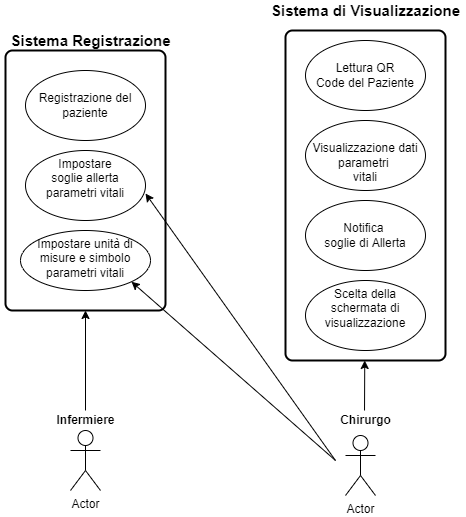
\includegraphics[width=11cm]{casiUso.png}
    \centering
    \caption{\label{pic:use-cases}Casi d'uso del sistema.}
\end{figure}

\subsubsection{Accesso del paziente in ospedale}
Quando il paziente deve essere ricoverato in ospedale è necessario registrarlo nel sistema informatico dell'ospedale. L'operatore incaricato dovrà quindi creare la sua cartella clinica compilando i dati richiesti. Successivamente, il chirurgo se lo ritiene necessario può configurare le soglie di allerta per i parametri vitali e infine verrà generato il relativo QR code che sarà utilizzato per il riconoscimento del paziente in sala operatoria.

\subsubsection{Intervento chirurgico}
Se è necessario eseguire un operazione chirurgica al paziente, il chirurgo può utilizzare oltre al monitor a parametri vitali fisico anche quello virtuale grazie alla visualizzazione di un ologramma. Per fare ciò sarà necessario scannerizzare il QR code del paziente (generato in fase di ricovero) sia nel monitor fisico sia nell'ologramma al fine di creare la connessione tra i due sistemi per la ricezione dei dati. In questo modo il chirurgo potrà visualizzare nell'ologramma i dati relativi ai parametri vitali del paziente, eventuali allarmi, i grafici, i valori puntuali e scegliere di monitorare un preciso parametro anziché avere una schermata generale di tutti. Inoltre sarà possibile visualizzare la cartella clinica del paziente compilata in fase di ricovero.

\subsection{Non funzionali}
I requisiti non funzionali sono così descritti.

\subsubsection{Usabilità}
l sistema deve fornire agli utenti finali un’interfaccia chiara, semplice, ben organizzata in modo da poter utilizzare al meglio tutte le sue funzionalità messe a disposizione e visualizzate.

\subsubsection{Legati al Sistema}
\begin{itemize}
    \item \textbf{Reattività}. L'utente non deve percepire ritardi tra la visualizzazione dei dati nel monitor a parametri vitali fisico e la visualizzazione degli stessi nell'ologramma;
    
    \item \textbf{Fault tolerance}. Deve essere implementato un adeguato sistema di gestione degli errori affinché le interruzioni involontarie non compromettono la salute del paziente durante un intervento chirurgico;
    
    \item \textbf{Sicurezza}. Utilizzando \textit{Azure Digital Twins} i dati salvati nel cloud e quelli in transito tra due o più componenti di Azure sono crittografati;
    
    \item \textbf{Scalabilità}. L’applicativo deve necessariamente consentire di aumentare o diminuire il numero di pazienti gestiti senza influire negativamente sulla prestazione del sistema. 
\end{itemize}

\subsection{Implementativi}
Il software dovrà essere realizzato utilizzando la filosofia \textit{Domain Driven Design}. Dovranno inoltre essere utilizzate metodologie di DevOps al fine di automatizzare e integrare quanti più processi possibili. Si utilizzerà il servizio Azure Digital Twins (PaaS - Platform As A Service) per la gestione dei digital twins e l'interfacciamento con i diversi clients. Per la parte di mixed reality si utilizzerà Unity e i visori Microsoft Hololens.

\section{Aspetti di Domain Driven Design}

\subsection{Core-Domain}
\subsection{Sub-Domain}
\subsection{Bounded Context}
\subsection{Context Map}